\documentclass[12pt]{article}
\usepackage[english]{babel}
\usepackage{natbib}
\usepackage{url}
\usepackage[utf8x]{inputenc}
\usepackage{amsmath}
\usepackage{color}
\usepackage{graphicx}
\graphicspath{{images/}}
\usepackage{parskip}
\usepackage{fancyhdr}
\usepackage{vmargin}
\setmarginsrb{3 cm}{2.5 cm}{3 cm}{2.5 cm}{1 cm}{1.5 cm}{1 cm}{1.5 cm}

\title{Resolving MDP domain problem using Q-learning algorithm with linear function approximation}			% Title
\author{Horpynchenko, Dmytro} 								% Author
\date{\today}											% Date

\makeatletter
\let\thetitle\@title
\let\theauthor\@author
\makeatother

\pagestyle{fancy}
\fancyhf{}

\lhead{\thetitle}
\cfoot{\thepage}

\begin{document}

%%%%%%%%%%%%%%%%%%%%%%%%%%%%%%%%%%%%%%%%%%%%%%%%%%%%%%%%%%%%%%%%%%%%%%%%%%%%%%%%%%%%%%%%%

\begin{titlepage}
	\centering
    
\includegraphics[scale = 0.2]{images/sapienza_logo_only.png}\\[1.0 cm]	% University Logo
    \textsc{\LARGE Sapienza University of Rome}\\[2.0 cm]	% University Name
	\textsc{\Large 1052217}\\[0.5 cm]				% Course Code
	\textsc{\large Artificial Intelligence}\\[0.5 cm]				% Course Name
	\rule{\linewidth}{0.2 mm} \\[0.4 cm]
	{ \huge \bfseries \thetitle}\\
	\rule{\linewidth}{0.2 mm} \\[1.5 cm]

	\begin{minipage}{0.4\textwidth}
		\begin{flushleft} \large
			\emph{Author:}\\
			\theauthor
			\end{flushleft}
			\end{minipage}~
			\begin{minipage}{0.4\textwidth}
			\begin{flushright} \large
			\emph{Student Number:} \\
			1807584				% Your Student Number
		\end{flushright}
	\end{minipage}\\[2 cm]


	\vfill

\end{titlepage}

%%%%%%%%%%%%%%%%%%%%%%%%%%%%%%%%%%%%%%%%%%%%%%%%%%%%%%%%%%%%%%%%%%%%%%%%%%%%%%%%%%%%%%%%%

\tableofcontents
\pagebreak

%%%%%%%%%%%%%%%%%%%%%%%%%%%%%%%%%%%%%%%%%%%%%%%%%%%%%%%%%%%%%%%%%%%%%%%%%%%%%%%%%%%%%%%%%

\section{Reinforcement learning}{}
\subsection{Overview}
\subsection{Marcov Decision Process}
\subsection{Properties}{policy, value function, q function, optimal policy}
\newpage
\section{Project domain} 
\subsection{Overview}{A car is on a one-dimensional track, positioned between two "mountains". The goal is to drive up the mountain on the right; however, the car's engine is not strong enough to scale the mountain in a single pass. Therefore, the only way to succeed is to drive back and forth to build up momentum (Figure~\ref{domain_image}).\par
The mountain car problem appeared first in Andrew Moore's PhD Thesis (1990). It was later more strictly defined in Singh and Sutton's Reinforcement Leaning paper with eligibility traces. The problem became more widely studied when Sutton and Barto added it to their book Reinforcement Learning: An Introduction (1998).\par
\begin{figure}[h!]
\begin{center}
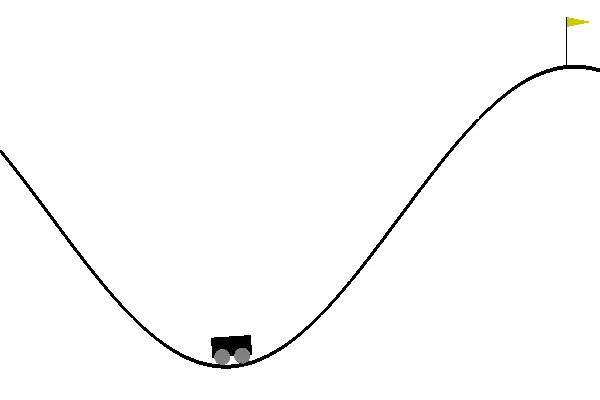
\includegraphics[scale=0.5]{images/domain.jpg}
\end{center}
\caption{Mounting car domain}
\label{domain_image}
\end{figure}
}
\subsection{GYM library}{
As a model of the domain was used GYM library (\url{https://gym.openai.com}), which contain list of environments such as classical "Inverted pendulum swing up" domain, "Atari" computer games, environments with physical world simulation.\par
Each environment communicate with algorithm through observation, action and reward .}
\subsection{Test domain specifications}
\label{subsec:spec}{
Output contains 2 continuous values of speed and acceleration in ranges [-0.7, 0.7] and [-0.7, 0.7] accordingly.\par
Input is discrete action id A={0, 1, 2}, where 0 - no action, 1 - move back, 2 - move forward.\par
To process action and obtain new state observation agent must call step() function. As a result, environment returns a tuple with new state observation, reward receiver from environment and boolean episode termination value.

}

\newpage
\section{Implementation}
\subsection{Project code structure}
\subsection{Agents}
\subsubsection{Random Agent}{For comparations and developmant purposes there was created agent that acts randomly.}
\subsubsection{State-action table agent}{To determine value of Q-function for every state-action pair agent use a table of finite size.\par
Since, as desribed in Section~\ref{subsec:spec}, domain has continuous output of speed and acceleration. Thus, observation received from domain discretized into natural numeric value in range [0, 40].\par
In such a way, Q-values table has resulting size of 40x40x3 of floating point values.
\subsubsection{Linear function approximation}
\newpage
\section{Results}
\newpage
\section{Conclusions}

\newpage
\bibliographystyle{plain}
\bibliography{biblist}

\end{document}
